\documentclass[a4paper,11pt,dvipdfmx]{ujarticle}
% パッケージ
\usepackage{graphicx}
\usepackage{url}
% レイアウト指定を記述したファイルの読み込み
\input{layout}

% タイトルと氏名を変更せよ.
\title{日本におけるデジタル化の状況}
\author{G4M3042024 片野 翔太}
\begin{document}

\maketitle %ここにタイトルが入る

% ここから本文
% 節見出し: \section{}
% を使う
\section{ブロードバンドの整備状況}
OECDによるブロードバンド回線の普及に関する調査\cite{soumu}によると,
図1に示すように,日本における100人あたりのモバイルブロードバンドの加入者は 
190.5 で, 第1位になっている.
2位はエストニアで, 3位米国と続く.
\begin{figure}[htbp]
 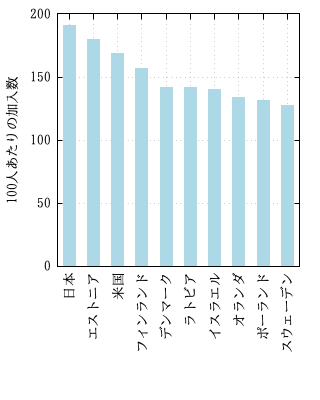
\includegraphics{fig21.png}
 \centering
 \caption{光ファイバー回線の加入者数(100人あたり)}
 \label{}
 \centering
\end{figure}
\section{デジタル競争力ランキング}
国際経営開発研究所(IMD)の調査\cite{imd}によると, 日本のデジタル競争力のランキングは
表\ref{tbl:利用状況}に示すように, 調査対象の64ヶ国中, 総合で28位, 技術分野で30位となっている.
\begin{table}[htbp]
    \centering
    \caption{デジタル競争力ランキング(64ヵ国中)}
    \label{tbl:利用状況}

   \begin{tabular}{|l|l|r|}\hline
           国    & 総合 & 技術\\
        \hline
          米国   & 1位& 4位\\
        \hline
          香港  & 2位 & 10位\\
        \hline
        スウェーデン& 3位 & 8位\\
        \hline
         デンマーク& 4位 & 2位 \\
        \hline
        シンガポール& 5位 & 3位\\
        \hline
    \end{tabular}

     \begin{tabular}{|l|l|r|}\hline
          韓国  \centering & 12位 & 13位\\
        \hline 
          中国  & 15位 & 20位\\
        \hline
    \end{tabular}

    \begin{tabular}{|l|l|r|}\hline
          日本  \centering & 28位 & 30位\\
        \hline
    \end{tabular} 

\end{table}

\section{考察}
\begin{itemize}
    \item 日本は世界の中では、通信インフラの分野については、力を入れている分野であると考えられる。
    \item 先進国の中で、日本は、デジタル競争力に関しては、劣っていることが分かるが、
    これの一つの要因として、国や地方公共団体などが、
    デジタル化の政策を進めてこなかったことが挙げられる。
    \item また米国については、Google, Amazon, Apple, Facebook, Microsoftなど,
    大手有名企業が集中するため、デジタルの競争力では、総合で1位となっていると考えられる。
\end{itemize}


% 本文(1)
%  参考文献の参照: \cite{}
%  図番号の参照: \ref{}
% を使う
% 文献データベースのキーワードは oecd と imd
% になっている.

% 図の挿入
% \includegraphics{}
% を
% \begin{figure}[htbp]
% \end{figure}
% で囲み
% \caption{}
% で図のタイトルを入れる.
% \label{}
% を使って図番号が参照できるようにする
% また,
% \centering
% で図が中央に来るようにする

% ーーー
% 節見出し(2)

% 本文(2)

% 表の挿入
% \begin{tabular}
% \end{tabular}    
% による表の記述を 
% \begin{table}[htbp]
% \end{table}
% で囲み
% \caption{}
% で表のタイトルを入れる.
% \label{}
% を使って表番号が参照できるようにする
% また,
% \centering
% で表が中央に来るようにする

% ーーー
% 見出し(3)
% 考察
%
% \begin{itemize}
% \end{itemize}
% を使って箇条書きで記述する

% ここに参考文献が入る
%
\bibliographystyle{junsrt}
\bibliography{exercise.bib}

\end{document}